\documentclass[12pt]{book}
\usepackage{graphicx}
\usepackage{amsmath}
\usepackage{hyperref}
\usepackage{geometry}
\usepackage{fontspec} % For custom fonts
\usepackage{xcolor}
\usepackage{float}
\usepackage{titling}
\usepackage{tikz}
\usepackage{fancyhdr} % For custom headers/footers
\usepackage{tocbibind} % To include TOC, LOF, LOT in TOC
\setmainfont{Times New Roman} % Set the main font to Times New Roman
\geometry{a4paper, margin=1in}
\usepackage{setspace}
\onehalfspacing 
\usepackage{titlesec}

\titleformat{\chapter}[display]
    {\normalfont\large\bfseries\centering}
    {\chaptertitlename\ \thechapter}
   {20pt}
    {\Large}

\titleformat{\section}
    {\normalfont\bfseries} 
    {\thesection}
    {1em}
    {}

\begin{document}
	\frontmatter
			 \pretitle{
				\begin{tikzpicture}[remember picture, overlay]
			   		\node[anchor=north west, xshift=1.5cm, yshift=-1cm] at (current page.north west) {
        						\includegraphics[width=2.5cm]{image1.png}
					};
    					\node[anchor=north west, xshift=4cm, yshift=-1cm] at (current page.north west) {
        						\includegraphics[width=2.3cm]{image2.png}
					};
					\node[anchor=north east, xshift=-1.5cm, yshift=-1cm] at (current page.north east) {
        						
\includegraphics[width=5cm]{image3.png}
					};
				\end{tikzpicture}
				\begin{center}
					\textbf{\large UNIVERSITE DE FIANARANTSOA ECOLE NATIONALE D'INFORMATIQUE \\[0.5cm] MEMOIRE DE FIN D'ETUDES POUR L'OBTENTION DU DIPLOME DE MASTER PROFESSIONNELLE}
					\\[0.5cm]
							\textbf{\underline{Mention:}} Informatique \\	
							\textbf{\underline{Parcours:}} Informatique générale\\
							\textbf{\textit{Intitulé}}				\end{center}
				\begin{center}\large\bfseries
			}
			\preauthor{\begin{flushleft}\fontsize{12} \lineskip Présenté le 01 février 2023\\ }
			\postauthor{\end{flushleft} \textbf{Membres du Jury:} \\ \begin{itemize}
			    \item \textbf{Président:} Monsieur RALAIVAO Jean Christian, Assistant d'Enseignement Supérieur et de Recherche;
			    \item \textbf{Examinateur:} Monsieur RALAIVAO Jean Christian, Assistant d'Enseignement Supérieur et de Recherche;
			    \item \textbf{Rapporteurs:} \begin{itemize}
       									 \item Monsieur RALAIVAO Jean Christian, Assistant d'Enseignement Supérieur et de Recherche;
       									 \item Monsieur RALAIVAO Jean Christian, Assistant d'Enseignement Supérieur et de Recherche.
    								\end{itemize}
			\end{itemize} }
			\predate{\begin{flushright} Année Universitaire: }
			\postdate{\end{flushright}}
			\title{
				\color{blue}
				\setlength{\fboxsep}{10pt} 
				\fbox{
					\begin{minipage}{\textwidth}
						\begin{center}
							CONCEPTION ET REALISATION  D'UNE APPLICATION WEB  DE RESERVATION DE VOYAGE
						\end{center}
					  \end{minipage}
				}
			}
			\author{\textbf{Par:} Monsieur ANDRIAMIORA Ainamalala Lucky}
			\date{2024-2025}
			\maketitle
			
			\newpage
			\thispagestyle{empty}
			\mbox{}

			\newpage
			\pagenumbering{roman}
			\renewcommand{\thepage}{\Roman{page}} % Ensure uppercase Roman numerals
			\setcounter{page}{1}
			\chapter*{CURRICULUM VITAE}
			\addcontentsline{toc}{chapter}{CURRICULUM VITAE}	
			\begin{minipage}{0.6\textwidth}
				\textbf{Nom:} ANDRIAMIORA\\
				\textbf{Prenom:} Ainamalala Lucky\\
				\textbf{Numéro:} +261 34 33 513 61\\
				\textbf{Addresse:} IIG20 E Ambatomaro, Antananarivo\\
				\textbf{E-mail:} luckyainamalalalucky@gmail.com\\
				\textbf{Date et lieu de naissance:} 30 décembre 1999 à Antsirabe
			\end{minipage}
			\hfill
			\begin{minipage}{0.3\textwidth}
				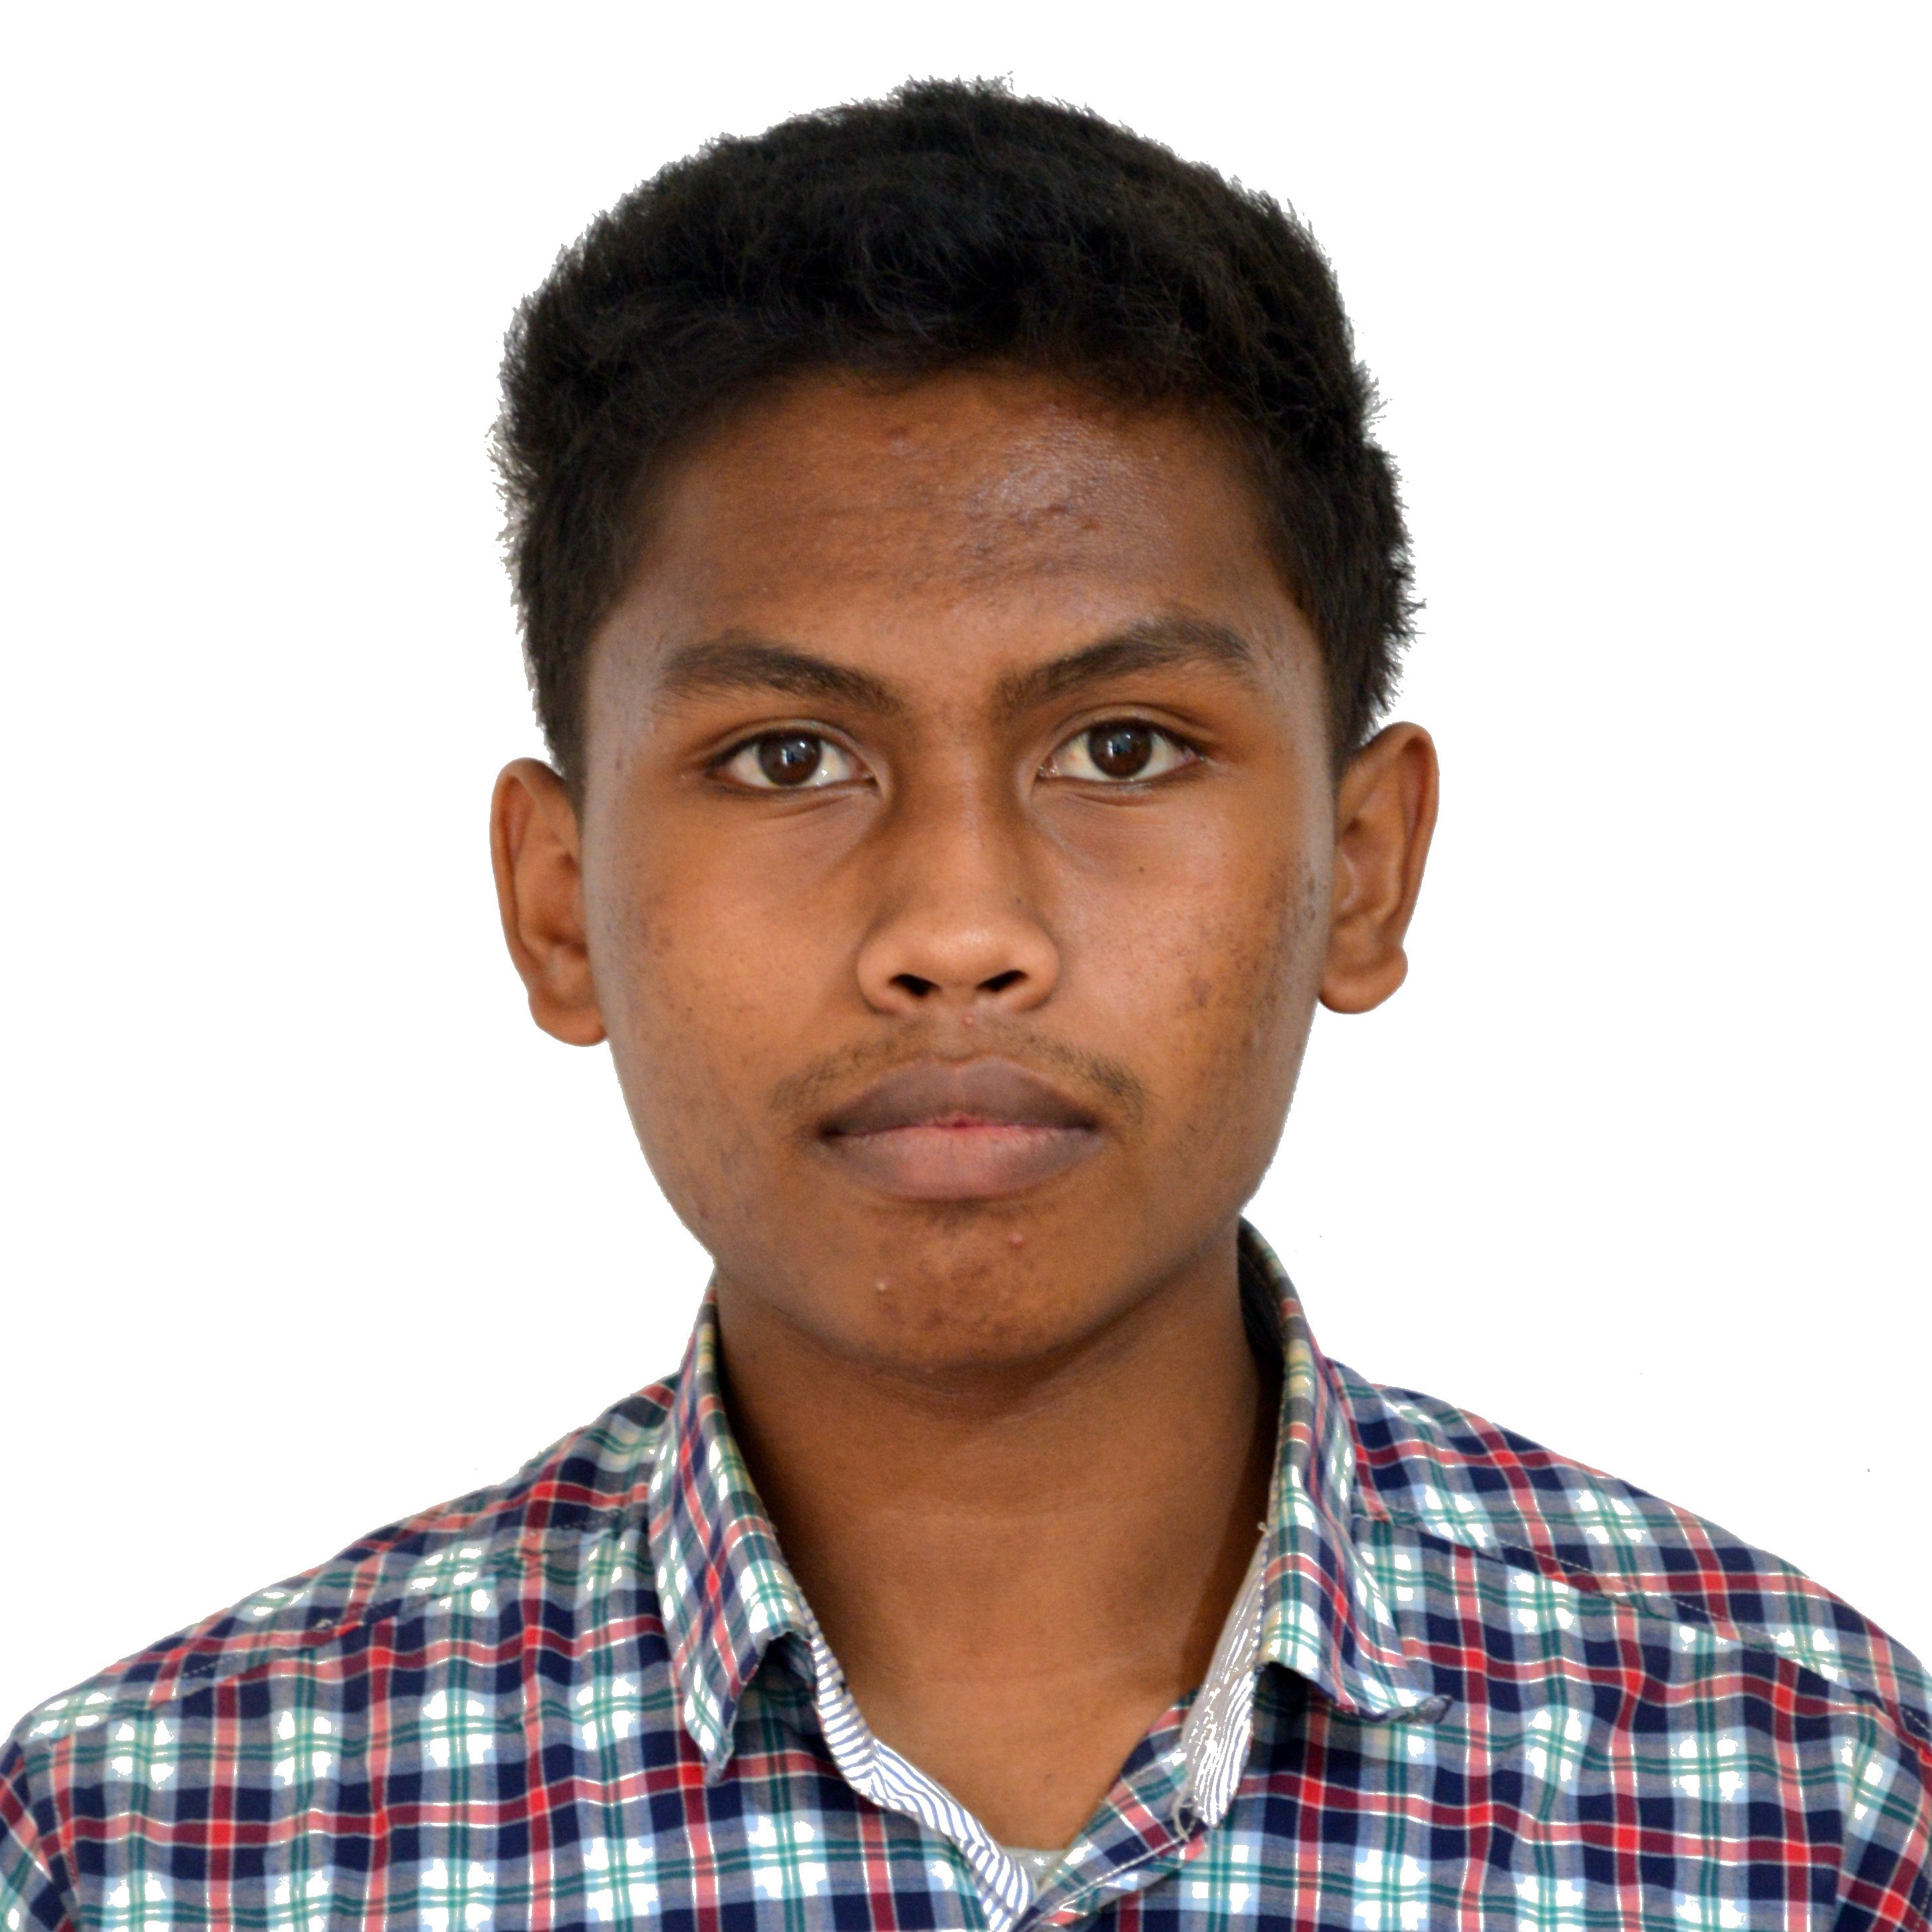
\includegraphics[width=3.5cm]{mypic.jpg}	
			\end{minipage}
			\section{FORMATIONS ET DIPLOME}
			\begin{minipage}{\textwidth}
				\textbf{2024-2025:} Deuxième année de formation en Master professionnelle à l’École Nationale d'Informatique, Université de Fianarantsoa . parcours : Informatique générale\\
				\textbf{2023-2024:} Première année de formation en Master professionnelle à l’École Nationale d'Informatique, Université de Fianarantsoa . parcours : Informatique générale\\
				\textbf{2022-2023:} Obtention du diplôme de Licence professionnelle mention Bien à l’École Nationale d'Informatique, Université de Fianarantsoa . parcours : Informatique générale\\
				\textbf{2021-2022:} Deuxième année de formation en Licence professionnelle à l’École Nationale d'Informatique, Université de Fianarantsoa . parcours : Informatique générale\\
				\textbf{2020-2021:} Première année de formation en Licence professionnelle à l’École Nationale d'Informatique, Université de Fianarantsoa . parcours : Informatique générale\\
				\textbf{2019-2020:} Obtention du diplôme de Baccalauréat série D mention assez-bien au Lycée André Résampa Antsirabe.
			\end{minipage}
			\section{STAGES ET EXPERIENCES PROFESSIONNELLES}
				\begin{minipage}{\textwidth}
       					 \textbf{19 octobre 2022 au 16 janvier 2023:} Stage auprès de la Paositra malagasy.
						\begin{itemize}
							\item \textbf{Thème du stage:} Application web pour la gestion des change;
							\item \textbf{Langages et outils:} Java, spring boot, Angular, TypeScript, PostgreSQL, UML.								
						\end{itemize}
    				\end{minipage}		
\end{document}